%\documentclass[smaller, handout]{beamer}
\def\bmode{0} % Mode 0 for presentation, mode 1 for a handout with notes, mode 2 fo% r handout without notes
\if 0\bmode
\documentclass[smaller]{beamer}
\else \if 1\bmode
\immediate\write18{pdflatex -jobname=\jobname-Handout-Notes\space\jobname}
\documentclass[smaller,handout]{beamer}
\usepackage{handoutWithNotes}
\pgfpagesuselayout{2 on 1 with notes}[letterpaper, landscape, border shrink=4mm]
\else \if 2\bmode
\immediate\write18{pdflatex -jobname=\jobname-Handout\space\jobname}
\documentclass[smaller,handout]{beamer}
\fi
\fi
\fi

%%%%%%%%%%%%%%%%%%%%%%%%%%%%%%%%%%%%%%%%%%%%%%%%%%%%%%%%%%%%%%%%%%%%%%%%%%%%%%%%%%%%%%%%%%%%%
\newcommand{\coursetitle}{CEE 616: Probabilistic Machine Learning}
\newcommand{\longlecturetitle}{M2 Deep Neural Networks:\\ Neural Networks for Structured Data II}
\newcommand{\shortlecturetitle}{L3b: NNs for Structured Data II}
\newcommand{\instructor}{Jimi Oke}
\newcommand{\lecturedate}{Tue, Oct 21, 2025}
%%%%%%%%%%%%%%%%%%%%%%%%%%%%%%%%%%%%%%%%%%%%%%%%%%%%%%%%%%%%%%%%%%%%%%%%%%%%%%%%%%%%%%%%%%%%%

 
 
% \usepackage[T1]{fontenc} 
% \usepackage{lmodern} 
%\usepackage{etex}
 %\newcommand{\num}{6{} }

% \usetheme[
%   outer/progressbar=foot,
%   outer/numbering=fraction,
%   block=fill,
%   inner/subsectionpage=progressbar
% ]{metropolis}
\usetheme{Madrid}
\useoutertheme[subsection=false]{miniframes} % Alternatively: miniframes, infolines, split
\useinnertheme{circles}
% %\useoutertheme{Frankfurt}
% \usecolortheme{beaver}
% %\useoutertheme{crane}
% %\useoutertheme{metropolis}
\usepackage[backend=biber,style=authoryear,maxcitenames=2,maxbibnames=99,safeinputenc,url=false, eprint=false]{biblatex}
%\addbibresource{bib/references.bib}
% \AtEveryCitekey{\iffootnote{{\tiny}\tiny}{\tiny}}

% %\usepackage{pgfpages}
% %\setbeameroption{hide notes} % Only slides
% %\setbeameroption{show only notes} % Only notes
% %\setbeameroption{hide notes} % Only notes
% %\setbeameroption{show notes on second screen=right} % Both

% % \usepackage[sfdefault]{Fira Sans}

% % \setsansfont[BoldFont={Fira Sans}]{Fira Sans Light}
% % \setmonofont{Fira Mono}

% %\usepackage{fira}
% %\setsansfont{Fira}
% %\setmonofont{Fira Mono}
% % To give a presentation with the Skim reader (http://skim-app.sourceforge.net) on OSX so
% % that you see the notes on your laptop and the slides on the projector, do the following:
% % 
% % 1. Generate just the presentation (hide notes) and save to slides.pdf
% % 2. Generate onlt the notes (show only nodes) and save to notes.pdf
% % 3. With Skim open both slides.pdf and notes.pdf
% % 4. Click on slides.pdf to bring it to front.
% % 5. In Skim, under "View -> Presentation Option -> Synhcronized Noted Document"
% %    select notes.pdf.
% % 6. Now as you move around in slides.pdf the notes.pdf file will follow you.
% % 7. Arrange windows so that notes.pdf is in full screen mode on your laptop
% %    and slides.pdf is in presentation mode on the projector.

% % Give a slight yellow tint to the notes page
% \setbeamertemplate{note page}{\pagecolor{yellow!5}\insertnote}\usepackage{palatino}

% %\usetheme{metropolis}
% %\usecolortheme{beaver}
 \usepackage{tipa}
% \usepackage{enumerate}
\definecolor{darkcandyapplered}{HTML}{A40000}
\definecolor{lightcandyapplered}{HTML}{e74c3c}

% %\setbeamercolor{title}{fg=darkcandyapplered}

% \definecolor{UBCblue}{rgb}{0.04706, 0.13725, 0.26667} % UBC Blue (primary)
% \definecolor{UBCgrey}{rgb}{0.3686, 0.5255, 0.6235} % UBC Grey (secondary)

% % \setbeamercolor{palette primary}{bg=darkcandyapplered,fg=white}
% % \setbeamercolor{palette secondary}{bg=darkcandyapplered,fg=white}
% % \setbeamercolor{palette tertiary}{bg=darkcandyapplered,fg=white}
% % \setbeamercolor{palette quaternary}{bg=darkcandyapplered,fg=white}
% % \setbeamercolor{structure}{fg=darkcandyapplered} % itemize, enumerate, etc
% % \setbeamercolor{section in toc}{fg=darkcandyapplered} % TOC sections
% % \setbeamercolor{frametitle}{fg=darkcandyapplered,bg=white} % TOC sections
% % \setbeamercolor{title in head/foot}{bg=white,fg=white} % TOC sections
% % \setbeamercolor{button}{fg=darkcandyapplered} % TOC sections

% % % Override palette coloring with secondary
% % \setbeamercolor{subsection in head/foot}{bg=lightcandyapplered,fg=white}

%\usecolortheme{crane}
% \makeatletter
% \setbeamertemplate{headline}{%
%   \begin{beamercolorbox}[colsep=1.5pt]{upper separation line head}
%   \end{beamercolorbox}
%   \begin{beamercolorbox}{section in head/foot}
%     \vskip1pt\insertsectionnavigationhorizontal{\paperwidth}{}{}\vskip1pt
%   \end{beamercolorbox}%
%   \ifbeamer@theme@subsection%
%     \begin{beamercolorbox}[colsep=1.5pt]{middle separation line head}
%     \end{beamercolorbox}
%     \begin{beamercolorbox}[ht=2.5ex,dp=1.125ex,%
%       leftskip=.3cm,rightskip=.3cm plus1fil]{subsection in head/foot}
%       \usebeamerfont{subsection in head/foot}\insertsubsectionhead
%     \end{beamercolorbox}%
%   \fi%
%   \begin{beamercolorbox}[colsep=1.5pt]{lower separation line head}
%   \end{beamercolorbox}
% }
% \makeatother

% Reduce size of frame box
\setbeamertemplate{frametitle}{%
    \nointerlineskip%
    \begin{beamercolorbox}[wd=\paperwidth,ht=2.0ex,dp=0.6ex]{frametitle}
        \hspace*{1ex}\insertframetitle%
    \end{beamercolorbox}%
}


%\setbeamercolor{frametitle}{bg=darkcandyapplered!80!black!90!white}
%\setbeamertemplate{frametitle}{\bf\insertframetitle}

%\setbeamercolor{footnote mark}{fg=darkcandyapplered}
%\setbeamercolor{footnote}{fg=darkcandyapplered!70}
%\Raggedbottom
%\setbeamerfont{page number in head/foot}{size=\tiny}
%\usepackage[tracking]{microtype}


% %\usepackage[sc,osf]{mathpazo}   % With old-style figures and real smallcaps.
% %\linespread{1.025}              % Palatino leads a little more leading

% % Euler for math and numbers
% %\usepackage[euler-digits,small]{eulervm}
% %\AtBeginDocument{\renewcommand{\hbar}{\hslash}}
\usepackage{graphicx}
\usepackage{multirow}
\usepackage{booktabs}
\usepackage{graphbox}
\usepackage{animate}
\usepackage{media9}
\usepackage{adjustbox}

% %\mode<presentation> { \setbeamercovered{transparent} }

\setbeamertemplate{navigation symbols}{}
\makeatletter
\def\beamerorig@set@color{%
  \pdfliteral{\current@color}%
  \aftergroup\reset@color
}
\def\beamerorig@reset@color{\pdfliteral{\current@color}}
\makeatother


% %=== GRAPHICS PATH ===========
\graphicspath{{./m5-images/}}
% % Marginpar width
% %Marginpar width
% %\setlength{\marginparsep}{.02in}


% %% Captions
% % \usepackage{caption}
% % \captionsetup{
% %   labelsep=quad,
% %   justification=raggedright,
% %   labelfont=sc
% % }

% \setbeamerfont{caption}{size=\footnotesize}
% \setbeamercolor{caption name}{fg=darkcandyapplered}

% %AMS-TeX packages

\usepackage{amssymb}
\usepackage{amsmath}
\usepackage{amsthm}
\usepackage{mathtools} 
\usepackage{bm}
\DeclareMathOperator*{\argmax}{arg\,max}
\DeclareMathOperator*{\argmin}{arg\,min}
% \usepackage{color}

% %https://tex.stackexchange.com/a/31370/2269
\usepackage{cancel}
\renewcommand{\CancelColor}{\color{red}} %change cancel color to red
\makeatletter
\let\my@cancelto\cancelto %copy over the original cancelto command
\newcommand<>{\cancelto}[2]{\alt#3{\my@cancelto{#1}{#2}}{\mathrlap{#2}\phantom{\my@cancelto{#1}{#2}}}}
% redefine the cancelto command, using \phantom to assure that the
% result doesn't wiggle up and down with and without the arrow
\makeatother


% % \usepackage{comment}
\usepackage{enumerate}
\usepackage{hyperref}
% \usepackage{minitoc,array}
% \definecolor{slblue}{rgb}{0,.3,.62}
\hypersetup{
    colorlinks,%
    citecolor=blue,%
    filecolor=blue,%
    linkcolor=blue,
    urlcolor=blue
}

% \usepackage{epstopdf}
% \epstopdfDeclareGraphicsRule{.gif}{png}{.png}{convert gif:#1 png:\OutputFile}
% \AppendGraphicsExtensions{.gif}

% %\usepackage{listings}

% %%% TIKZ
\usepackage{forest}
\usepackage{tikz}
\usepackage{tikz-3dplot}
\usepackage{pgfplots}
\usepackage{pgfplotstable}
% \usepackage{pgfgantt}
\usepackage{neuralnetwork}

\usetikzlibrary{fit,arrows,arrows.meta,shapes,positioning,shapes.geometric}
\usetikzlibrary{decorations.markings}
\usetikzlibrary{shadows,automata}
\usetikzlibrary{patterns}
\usetikzlibrary{trees,mindmap,backgrounds}
%\usetikzlibrary{circuits.ee.IEC}
\usetikzlibrary{decorations.text}
% % For Sagnac Picture
% \usetikzlibrary{%
%     decorations.pathreplacing,%
%     decorations.pathmorphing%
% }
% \tikzset{no shadows/.style={general shadow/.style=}}
% %
% %\usepackage{paralist}

\tikzset{
  font=\Large\sffamily\bfseries,
  red arrow/.style={
    midway,red,sloped,fill, minimum height=3cm, single arrow, single arrow head extend=.5cm, single arrow head indent=.25cm,xscale=0.3,yscale=0.15,
    allow upside down
  },
  black arrow/.style 2 args={-stealth, shorten >=#1, shorten <=#2},
  black arrow/.default={1mm}{1mm},
  tree box/.style={draw, rounded corners, inner sep=1em},
  node box/.style={white, draw=black, text=black, rectangle, rounded corners},
}

% %%% FORMAT PYTHON CODE
% %\usepackage{listings}
% % Default fixed font does not support bold face
% \DeclareFixedFont{\ttb}{T1}{txtt}{bx}{n}{8} % for bold
% \DeclareFixedFont{\ttm}{T1}{txtt}{m}{n}{8}  % for normal

% % Custom colors
% \definecolor{deepblue}{rgb}{0,0,0.5}
% \definecolor{deepred}{rgb}{0.6,0,0}
% \definecolor{deepgreen}{rgb}{0,0.5,0}

% %\usepackage{animate}

% % Python style for highlighting
% % \newcommand\pythonstyle{\lstset{
% % language=Python,
% % basicstyle=\footnotesize\ttm,
% % otherkeywords={self},             % Add keywords here
% % keywordstyle=\footnotesize\ttb\color{deepblue},
% % emph={MyClass,__init__},          % Custom highlighting
% % emphstyle=\footnotesize\ttb\color{deepred},    % Custom highlighting style
% % stringstyle=\color{deepgreen},
% % frame=tb,                         % Any extra options here
%     % showstringspaces=false            % 
% % }}

% % % Python environment
% % \lstnewenvironment{python}[1][]
% % {
% % \pythonstyle
% % \lstset{#1}
% % }
% % {}

% % % Python for external files
% % \newcommand\pythonexternal[2][]{{
% % \pythonstyle
% % \lstinputlisting[#1]{#2}}}

% % Python for inline
% % 
% % \newcommand\pythoninline[1]{{\pythonstyle\lstinline!#1!}}

% %\usepackage{algorithm2e}

\newcommand{\eps}{\epsilon}
\newcommand{\bX}{\mb X}
\newcommand{\by}{\mb y}
\newcommand{\bbe}{\bm\beta}
\newcommand{\beps}{\bm\epsilon}
\newcommand{\bY}{\mb Y}

\newcommand{\osn}{\oldstylenums}
\newcommand{\dg}{^{\circ}}
\newcommand{\lt}{\left}
\newcommand{\rt}{\right}
\newcommand{\pt}{\phantom}
\newcommand{\tf}{\therefore}
\newcommand{\?}{\stackrel{?}{=}}
\newcommand{\fr}{\frac}
\newcommand{\dfr}{\dfrac}
\newcommand{\ul}{\underline}
\newcommand{\tn}{\tabularnewline}
\newcommand{\nl}{\newline}
\newcommand\relph[1]{\mathrel{\phantom{#1}}}
\newcommand{\cm}{\checkmark}
\newcommand{\ol}{\overline}
\newcommand{\rd}{\color{red}}
\newcommand{\bl}{\color{blue}}
\newcommand{\pl}{\color{purple}}
\newcommand{\og}{\color{orange!90!black}}
\newcommand{\gr}{\color{green!40!black}}
\newcommand{\lbl}{\color{CornflowerBlue}}
\newcommand{\dca}{\color{darkcandyapplered}}
\newcommand{\nin}{\noindent}
\newcommand*\circled[1]{\tikz[baseline=(char.base)]{
            \node[shape=circle,draw,thick,inner sep=1pt] (char) {\small #1};}}

\newcommand{\bc}{\begin{compactenum}[\quad--]}
\newcommand{\ec}{\end{compactenum}}

\newcommand{\p}{\partial}
\newcommand{\pd}[2]{\frac{\partial{#1}}{\partial{#2}}}
\newcommand{\dpd}[2]{\dfrac{\partial{#1}}{\partial{#2}}}
\newcommand{\pdd}[2]{\frac{\partial^2{#1}}{\partial{#2}^2}}
\newcommand{\pde}[3]{\frac{\partial^2{#1}}{\partial{#2}\partial{#3}}}
\newcommand{\nmfr}[3]{\Phi\left(\frac{{#1} - {#2}}{#3}\right)}
\newcommand{\Err}{\text{Err}}
\newcommand{\err}{\text{err}}

\DeclarePairedDelimiter\ceil{\lceil}{\rceil}
\DeclarePairedDelimiter\floor{\lfloor}{\rfloor}

%%%% GREEK LETTER SHORTCUTS %%%%%
\newcommand{\la}{\lambda}
\renewcommand{\th}{\theta}
\newcommand{\al}{\alpha}
\newcommand{\G}{\Gamma}
\newcommand{\si}{\sigma}
\newcommand{\Si}{\Sigma}


\pgfmathdeclarefunction{poiss}{1}{%
  \pgfmathparse{(#1^x)*exp(-#1)/(x!)}%
  }

\pgfmathdeclarefunction{gauss}{2}{%
  \pgfmathparse{1/(#2*sqrt(2*pi))*exp(-((x-#1)^2)/(2*#2^2))}%
}

\pgfmathdeclarefunction{expo}{2}{%
  \pgfmathparse{#1*exp(-#1*#2)}%
}

\pgfmathdeclarefunction{expocdf}{2}{%
  \pgfmathparse{1 -exp(-#1*#2)}%
}

\newcommand{\mb}{\mathbb}
\newcommand{\mc}{\mathcal}
\newcommand{\tr}{^{\top}}
\newcommand{\empt}[2]{$#1^{( #2 )}$}
\newcommand{\pe}{\pause}
% \usepackage{pst-plot}

% \usepackage{pstricks-add}
% \usepackage{auto-pst-pdf}   

% \psset{unit = 3}

% \def\target(#1,#2){%
%  {\psset{fillstyle = solid}
%   \rput(#1,#2){%
%     \pscircle[fillcolor = white](0.7,0.7){0.7}
%     \pscircle[fillcolor = blue!60](0.7,0.7){0.5}
%     \pscircle[fillcolor = white](0.7,0.7){0.3}
%     \pscircle[fillcolor = red!80](0.7,0.7){0.1}}}}
% \def\dots[#1](#2,#3){%
%     \psRandom[
%       dotsize = 2pt,
%       randomPoints = 25
%     ](!#2 #1 0.04 sub sub #3 #1 0.04 sub sub)%
%      (!#2 #1 0.04 sub add #3 #1 0.04 sub add)%
%      {\pscircle[linestyle = none](#2,#3){#1}}}


%%%%%%%%%%%%%%%%%%%%%%%%%%%%%%%%%%%%%%%%%%%%%%%%%%%
%%%%%%%%%%%%%%%%%%%%%%%%%%%%%%%%%%%%%%%%%%%%%%%%%%%
\title[\shortlecturetitle]{ {\normalsize \coursetitle}
  \\ \longlecturetitle}
\date[\lecturedate]{\footnotesize \lecturedate}
\author{{\bf \instructor}}
\institute[UMass Amherst]{
%\titlegraphic{\hfill
  \begin{tikzpicture}[baseline=(current bounding box.center)]
    \node[anchor=base] at (-7,0) (its) {\includegraphics[scale=.3]{UMassEngineering_vert}} ;
  \end{tikzpicture}
  % \hfill\includegraphics[height=1.5cm]{logo}
}

%https://tex.stackexchange.com/questions/55806/mindmap-tikzpicture-in-beamer-reveal-step-by-step
  \tikzset{
    invisible/.style={opacity=0},
    visible on/.style={alt={#1{}{invisible}}},
    alt/.code args={<#1>#2#3}{%
      \alt<#1>{\pgfkeysalso{#2}}{\pgfkeysalso{#3}} % \pgfkeysalso doesn't change the path
    },
  }


% https://tex.stackexchange.com/questions/446468/labels-with-arrows-for-an-equation
% https://tex.stackexchange.com/a/402466/121799
\newcommand{\tikzmark}[3][]{
\ifmmode
\tikz[remember picture,baseline=(#2.base)] \node [inner sep=0pt,#1](#2) {$#3$};
\else
\tikz[remember picture,baseline=(#2.base)] \node [inner sep=0pt,#1](#2) {#3};
\fi
}

% \lstset{language=matlab,
%                 basicstyle=\scriptsize\ttfamily,
%                 keywordstyle=\color{blue}\ttfamily,
%                 stringstyle=\color{blue}\ttfamily,
%                 commentstyle=\color{gray}\ttfamily,
%                 morecomment=[l][\color{gray}]{\#}
%               }


%%% Local Variables:
%%% mode: latex
%%% TeX-master: t
%%% End:

              
\begin{document}
\maketitle
\begin{frame}
  \frametitle{Outline}
  \tableofcontents
\end{frame}

 

 

\section{Backpropagation}
\begin{frame}
  \frametitle{Forward mode differentiation}
  \pause
  Let us think of a simple feedforward with inputs $\bm x =\bm x_1 \in \mathbb{R}^{D=4}$, 3 hidden layers with
   $m_1=8$, $m_2=6$, and $m_3=4$ neurons, and outputs $\bm o\in \mathbb{R}^2$:\pause

  \begin{center}
    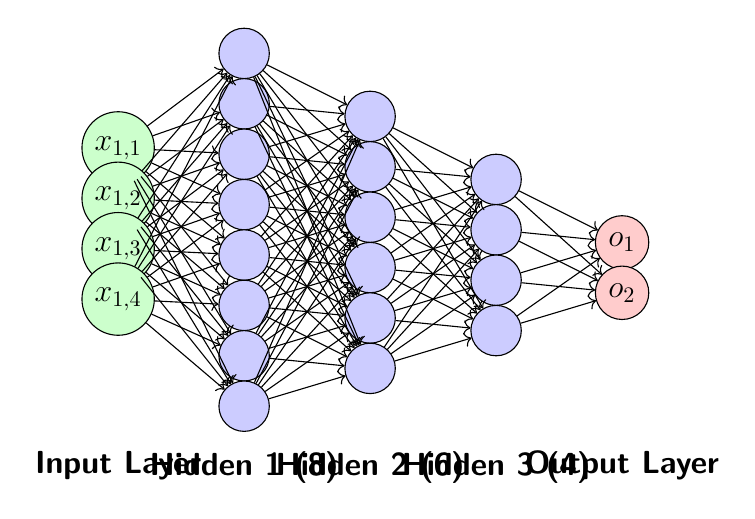
\begin{tikzpicture}[
      node distance=1.5cm and 2cm,
      neuron/.style={circle,draw,minimum size=8mm,fill=blue!20},
      input/.style={circle,draw,minimum size=8mm,fill=green!20},
      output/.style={circle,draw,minimum size=8mm,fill=red!20},
      layer/.style={rectangle,draw=none,minimum height=6cm,minimum width=1cm},
      scale=.8, transform shape
    ]

    % Input layer
    \foreach \i in {1,...,4}
      \node[input] (I\i) at (0, {3-0.8*\i}) {$x_{1,\i}$};

    % Hidden layer 1 (8 units)
    \foreach \i in {1,...,8}
      \node[neuron] (H1\i) at (2, {4.5-0.8*\i}) {};

    % Hidden layer 2 (6 units)
    \foreach \i in {1,...,6}
      \node[neuron] (H2\i) at (4, {3.5-0.8*\i}) {};

    % Hidden layer 3 (4 units)
    \foreach \i in {1,...,4}
      \node[neuron] (H3\i) at (6, {2.5-0.8*\i}) {};

    % Output layer (2 units)
    \foreach \i in {1,2}
      \node[output] (O\i) at (8, {1.5-0.8*\i}) {$o_\i$};

    % Connections input to hidden layer 1
    \foreach \i in {1,...,4}
      \foreach \j in {1,...,8}
        \draw[->] (I\i) -- (H1\j);

    % Connections hidden layer 1 to hidden layer 2
    \foreach \i in {1,...,8}
      \foreach \j in {1,...,6}
        \draw[->] (H1\i) -- (H2\j);

    % Connections hidden layer 2 to hidden layer 3
    \foreach \i in {1,...,6}
      \foreach \j in {1,...,4}
        \draw[->] (H2\i) -- (H3\j);

    % Connections hidden layer 3 to output
    \foreach \i in {1,...,4}
      \foreach \j in {1,2}
        \draw[->] (H3\i) -- (O\j);

    % Layer labels
    \node[below] at (0,-2.5) {Input Layer};
    \node[below] at (2,-2.5) {Hidden 1 (8)};
    \node[below] at (4,-2.5) {Hidden 2 (6)};
    \node[below] at (6,-2.5) {Hidden 3 (4)};
    \node[below] at (8,-2.5) {Output Layer};

    \end{tikzpicture}
  \end{center}

  \pause
  We consider each hidden unit as a function $\bm f_{\ell}(\cdot)$, where $\ell$ is the layer index, that maps the input $\bm x_{\ell}$ to the output of the hidden unit $\bm x_{\ell+1}$. \pause

\end{frame}


\begin{frame}
  \frametitle{Function composition}

  We can then express the output of the network as a composition of functions:

  \begin{eqnarray}
    \bm o &=& \bm f(\bm x)
  \end{eqnarray}

  \pause
  where 
  \begin{equation}
    \bm f = \bm f_{4} \circ \bm f_{3} \circ \bm f_{2} \circ \bm f_{1}
  \end{equation}

  and thus

  \begin{equation}
    \bm o = \bm f_{4}(\bm f_{3}(\bm f_{2}(\bm f_{1}(\bm x))))
  \end{equation}

  and
  \begin{eqnarray*}
    \bm x_{2} &=& \bm f_{1}(\bm x_1), \quad \bm f_1 : \mathbb{R}^4 \to \mathbb{R}^8 \\
    \bm x_{3} &=& \bm f_{2}(\bm x_{2}), \quad \bm f_2 : \mathbb{R}^8 \to \mathbb{R}^6 \\
    \bm x_4 &=& \bm f_{3}(\bm x_{3}), \quad \bm f_3 : \mathbb{R}^6 \to \mathbb{R}^4 \\
    \bm o &=& \bm f_{4}(\bm x_{4}), \quad \bm f_4 : \mathbb{R}^4 \to \mathbb{R}^2
  \end{eqnarray*}
\end{frame}

\begin{frame}
  \frametitle{Computational graph}\pause

  We can further visualize the FFNN as a computational graph:\pause

  \begin{center}
    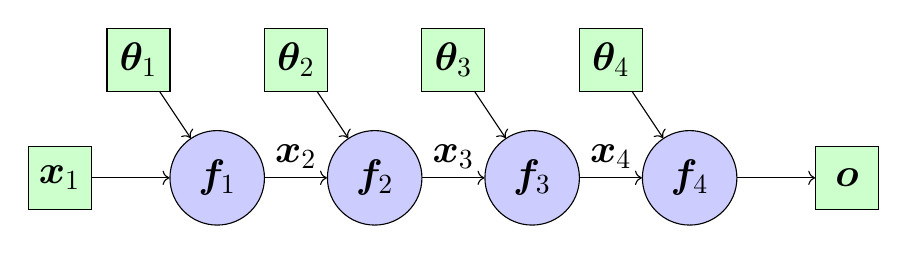
\begin{tikzpicture}[
      node distance=2cm,
      funcnode/.style={circle,draw,minimum size=12mm,fill=blue!20},
      datanode/.style={rectangle,draw,minimum size=8mm,fill=green!20},
      scale=1, transform shape
    ]

    % Input node
    \node[datanode] (x1) at (0, 0) {$\bm{x}_1$};

    % Function nodes
    \node[funcnode] (f1) at (2, 0) {$\bm{f}_1$};
    \node[funcnode] (f2) at (4, 0) {$\bm{f}_2$};
    \node[funcnode] (f3) at (6, 0) {$\bm{f}_3$};
    \node[funcnode] (f4) at (8, 0) {$\bm{f}_4$};

    % Output node
    \node[datanode] (o) at (10, 0) {$\bm{o}$};

    % Parameter nodes (coming from northwest)
    \node[datanode] (theta1) at (1, 1.5) {$\bm{\theta}_1$};
    \node[datanode] (theta2) at (3, 1.5) {$\bm{\theta}_2$};
    \node[datanode] (theta3) at (5, 1.5) {$\bm{\theta}_3$};
    \node[datanode] (theta4) at (7, 1.5) {$\bm{\theta}_4$};

    % Main flow arrows with labels
    \draw[->] (x1) -- (f1);
    \draw[->] (f1) -- (f2) node[midway,above] {$\bm{x}_2$};
    \draw[->] (f2) -- (f3) node[midway,above] {$\bm{x}_3$};
    \draw[->] (f3) -- (f4) node[midway,above] {$\bm{x}_4$};
    \draw[->] (f4) -- (o);

    % Parameter arrows from northwest
    \draw[->] (theta1) -- (f1);
    \draw[->] (theta2) -- (f2);
    \draw[->] (theta3) -- (f3);
    \draw[->] (theta4) -- (f4);

    \end{tikzpicture}
  \end{center}

  \pause
  where $\bm{\theta}_\ell$ are the parameters (weights and biases) of layer $\ell$.


\end{frame}

\begin{frame}
  \frametitle{Backpropagation}\pause

  To compute the gradient, we need to find:

  \begin{equation}
    \pd{\bm o}{\bm x} = \pd{\bm f_{4}(\bm x_{4})}{\bm x_{4}} \cdot \pd{\bm f_{3}(\bm x_{3})}{\bm x_{3}} \cdot \pd{\bm f_{2}(\bm x_{2})}{\bm x_{2}} \cdot \pd{\bm f_{1}(\bm x_{1})}{\bm x_{1}}
  \end{equation}

  \pause

  We define the Jacobian matrix of each layer as:
  \begin{equation}
    \bm J_{\bm f}(\bm x_{\ell}) = \pd{\bm f_{\ell}(\bm x_{\ell})}{\bm x_{\ell}} \pause
    = 
    \begin{pmatrix}
      \pd{f_{\ell,1}(\bm x_{\ell})}{x_{\ell,1}} & \pd{f_{\ell,1}(\bm x_{\ell})}{x_{\ell,2}} & \cdots & \pd{f_{\ell,1}(\bm x_{\ell})}{x_{\ell,D}} \\
      \pd{f_{\ell,2}(\bm x_{\ell})}{x_{\ell,1}} & \pd{f_{\ell,2}(\bm x_{\ell})}{x_{\ell,2}} & \cdots & \pd{f_{\ell,2}(\bm x_{\ell})}{x_{\ell,D}} \\
      \vdots & \vdots & \ddots & \vdots \\
      \pd{f_{\ell,M}(\bm x_{\ell})}{x_{\ell,1}} & \pd{f_{\ell,M}(\bm x_{\ell})}{x_{\ell,2}} & \cdots & \pd{f_{\ell,M}(\bm x_{\ell})}{x_{\ell,D}}
    \end{pmatrix}
  \end{equation}

  \pause
  Thus, the gradient of the output with respect to the input is given by:\pause
  \begin{equation}
    \pd{\bm o}{\bm x} = \bm J_{\bm f}(\bm x_{4}) \cdot \bm J_{\bm f}(\bm x_{3}) \cdot \bm J_{\bm f}(\bm x_{2}) \cdot \bm J_{\bm f}(\bm x_{1})
  \end{equation}
\end{frame}

\begin{frame}
  \frametitle{Jacobian matrix (2/2)}\pause

  We can write the Jacobian as:\pause

  \begin{equation}
    \bm J_{\bm f}(\bm x) = \pd{\bm f(\bm x)}{\bm x} =
    \begin{pmatrix}
    \nabla f_1(\bm x)\tr \\
    \nabla f_2(\bm x)\tr \\
    \vdots \\
    \nabla f_M(\bm x)\tr 
    \end{pmatrix} \pause = \lt( \pd{\bm f}{\bm x_1}, \pd{\bm f}{\bm x_2}, \ldots, \pd{\bm f}{\bm x_D} \rt)
  \end{equation}
\pause

\begin{itemize}
  \item $i$'th row: $\nabla f_i(\bm x)\tr \in \mb{R}^{1\times D}$ gradient of the $i$'th output w.r.t. all inputs
  \item $j$'th column: $\pd{\bm f}{x_j} \in\mb{R}^{M}$ gradient of all outputs w.r.t. the $j$'th input
\end{itemize}
  
\pause

Thus:
\begin{equation}
  \nabla \bm f(\bm x) = \bm J_{\bm f}(\bm x)\tr = \lt( \nabla f_1(\bm x), \nabla f_2(\bm x), \ldots, \nabla f_M(\bm x) \rt)
\end{equation}
\end{frame}

\begin{frame}
  \frametitle{Vector Jacobian product}\pause

  The vector-Jacobian product (VJP) is the left-multiplication of the Jacobian matrix $\bm J_{\bm f}(\bm x)$ by a vector $\bm u$, which results in a row vector:\pause
  \begin{equation}
    \bm u \tr \bm J_{\bm f}(\bm x) \in \mathbb{R}^{1\times D}
  \end{equation}

  \pause

  \begin{itemize}
    \item If $\bm u\in \mb{R}^{M}$ is a one-hot vector with 1 at index $i$ and 0 elsewhere, e.g.
      \begin{equation}
        \bm u = 
        \begin{pmatrix}
          0 \\ \vdots \\ 1 \\ \vdots \\ 0
        \end{pmatrix} = \bm e_i
      \end{equation}

        then the VJP $\bm e_i\tr \bm J_{\bm f}(\bm x)$ extracts the $i$'th row from $\bm J_{\bm f}(\bm x)$, which is the gradient of the $i$'th output with respect to all inputs, $\nabla f_i(\bm x)\tr$.

  \end{itemize}
\end{frame}

\begin{frame}
  \frametitle{Jacobian-vector product}\pause

  The Jacobian-vector product (JVP) is the right-multiplication of the Jacobian matrix $\bm J_{\bm f}(\bm x)$ by a vector $\bm v$, which results in a column vector:\pause

  \begin{equation}
    \bm J_{\bm f}(\bm x) \bm v \in \mathbb{R}^{M}
  \end{equation}

  \pause
\begin{itemize}
  \item If $\bm v\in \mb{R}^{D}$ is a one-hot vector with 1 at index $j$ and 0 elsewhere, e.g.
      \begin{equation}
        \bm v = 
        \begin{pmatrix}
          0 \\ \vdots \\ 1 \\ \vdots \\ 0
        \end{pmatrix} = \bm e_j
      \end{equation}

        then the JVP $\bm J_{\bm f}(\bm x) \bm e_j$ extracts the $j$'th column from $\bm J_{\bm f}(\bm x)$, which is the gradient of all outputs with respect to the $j$'th input, $\pd{\bm f}{x_j}$.
\end{itemize}
\end{frame}

\begin{frame}
  \frametitle{Computing the Jacobian}\pause

  \begin{itemize}
    \item The Jacobian can be computed by performing either $M$ JVPs (one per input dimension) or $D$ VJPs (one per output dimension)
    \item If $D < M$, it is more efficient to compute the Jacobian via JVPs for each column $j$:
      \begin{equation}
        \bm J_{\bm f}(\bm x)(\bm v) = \underbrace{\bm J_{\bm f}(\bm x)_4}_{M \times M_3} \underbrace{\bm J_{\bm f}(\bm x)_3}_{M_3 \times M_2} \underbrace{\bm J_{\bm f}(\bm x)_2}_{M_2 \times M_1} \underbrace{\bm J_{\bm f}(\bm x)_1}_{M_1 \times D} \underbrace{\bm v}_{D \times 1}
      \end{equation}
      in a right-to-left fashion (\textbf{forward mode differentiation})
    \item If $M < D$, it is more efficient to compute the Jacobian via VJPs for each row $i$:
      \begin{equation}
        \bm u\tr \bm J_{\bm f}(\bm x) = \underbrace{\bm u\tr}_{1 \times M} \underbrace{\bm J_{\bm f}(\bm x)_4}_{M \times M_3} \underbrace{\bm J_{\bm f}(\bm x)_3}_{M_3 \times M_2} \underbrace{\bm J_{\bm f}(\bm x)_2}_{M_2 \times M_1} \underbrace{\bm J_{\bm f}(\bm x)_1}_{M_1 \times D}
      \end{equation}
      in a left-to-right fashion (\textbf{reverse mode differentiation})
    \item In neural networks, the number of outputs $M$ is often much smaller than the number of inputs $D$
    \item Thus, backpropagation typically employs VJPs to compute the gradients efficiently
  \end{itemize}
\end{frame}

\begin{frame}
  \frametitle{Example: single hidden layer MLP}\pause

  Consider a single hidden layer MLP with an $\ell_2$ loss for regression (scalar output):\pause
  \begin{equation}
    \mc{L}((\bm x, \bm y),\bm\th) = \fr12 ||\bm y - \bm W_2\varphi(\bm W_1\bm x)||_2^2
  \end{equation}
  \pause
  We can represent the network as follows:\pause
  \begin{eqnarray}
    \mc L &=& \bm f_4 \circ \bm f_3 \circ \bm f_2 \circ \bm f_1  \\\pause
    \bm x_2 &=& \bm f_1(\bm x, \bm\th_1) = \bm W_1 \bm x \\\pause
    \bm x_3 &=& \bm f_2(\bm x_2, \bm\th_2) = \varphi(\bm x_2) \\\pause
    \bm x_4 &=& \bm f_3(\bm x_3, \bm\th_3) = \bm W_2 \bm x_3 \\\pause
    \mc L &=& \bm f_4(\bm x_4, \bm y) = \fr12||\bm y - \bm x_4||_2^2
  \end{eqnarray}
  and $\mc L : \mathbb{R}^D \to \mathbb{R}$.
\end{frame}
\begin{frame}
  \frametitle{Example: single hidden layer MLP (contd.)}\pause

  Using the chain rule, We can express the gradient of the loss wrt the parameters in each layer as:\pause
  \begin{eqnarray}
    \pd{\mc L}{\bm\th_3} &=& \pd{\mc L}{\bm x_4} \pd{\bm x_4}{\bm\th_3} \\\pause
    \pd{\mc L}{\bm\th_2} &=& \pd{\mc L}{\bm x_4} \pd{\bm x_4}{\bm x_3} \pd{\bm x_3}{\bm\th_2} \\ \pause
    \pd{\mc L}{\bm\th_1} &=& \pd{\mc L}{\bm x_4} \pd{\bm x_4}{\bm x_3} \pd{\bm x_3}{\bm x_2} \pd{\bm x_2}{\bm\th_1}
  \end{eqnarray}
  \pause
  Note:
  \begin{equation}
    \pd{\mc L}{\bm\th_k} = \lt(\nabla_{\bm\th_k} \mc L\rt)\tr
  \end{equation}
  is a $d_k$-dimensional gradient row vector, where $d_k$ is the number of parameters in layer $k$ \pause and can be computed recursively as VJPs:
  \begin{equation}
    \pd{\mc L}{\bm\th_k} = \bm u_{k+1}\tr \pd{\bm f_k(\bm x_k, \bm\th_k)}{\bm\th_k}
  \end{equation}
  where $\bm x_{k+1} = \bm f_k(\bm x_k, \bm\th_k)$, $\bm u_{k}\tr = \bm u_{k+1}\tr\pd{\bm f_k(\bm x_k, \bm\th_k)}{\bm x_{k}}$ and $\bm u_{K+1} = 1$.
\end{frame}

\begin{frame}
  \frametitle{Example: single hidden layer MLP (contd.)}\pause
We then need to specify the Jacobians for each layer:\pause
\begin{itemize}
\item Output layer:
  \begin{eqnarray}
    \pd{\mc L}{\bm x_4} &=& \bm u_4\tr = \pd{\fr12||\bm y - \bm x_4||_2^2}{\bm x_4} = (\bm x_4 - \bm y)\tr
  \end{eqnarray}
  \pause
  \item Linear layer:
    \begin{eqnarray}
    \pd{\bm x_4}{\bm x_3} &=& \bm J_{\bm f_3}(\bm x_3) = \pd{\bm W_2 \bm x_3}{\bm x_3} = \bm W_2 \\
    \pd{\bm x_4}{\bm W_2} &=& \pd{\bm W_2 \bm x_3}{\bm W_2} = \bm x_3\tr
  \end{eqnarray}
  \pause

  % \item Activation layer:
  %   \begin{eqnarray}
  %   \pd{\bm x_3}{\bm x_2} &=& \bm J_{\bm f_2}(\bm x_2) = \pd{\varphi(\bm x_2)}{\bm x_2} = \diag\lt(\varphi'(\bm x_2)\rt) \\
  %   \pd{\bm x_3}{\bm\th_2} &=& 0
  % \end{eqnarray}
  % \pause
  % \item Linear layer:
  %   \begin{eqnarray}
  %   \pd{\bm x_2}{\bm x_1} &=& \bm J_{\bm f_1}(\bm x_1) = \pd{\bm W_1 \bm x_1}{\bm x_1} = \bm W_1 \\
  %   \pd{\bm x_2}{\bm W_1} &=& \pd{\bm W_1 \bm x_1}{\bm W_1} = \bm x_1\tr
  % \end{eqnarray}  
\end{itemize} 
\end{frame}


\section{Training}
\begin{frame}
  \frametitle{Batch learning}
  The gradient descent method was described without referencing the observations. \pause

  \medskip

  In reality, the forward and backward passes are performed for each observation in the training set, with parameter updates obtained by
  \textbf{\bl averaging} the gradients: \pause

  \begin{eqnarray}
    \bm\th_{\ell, t+1}  &=& \pause  \bm\th_{\ell,t} - \pause \rho{\bl  \fr1N \sum_{n=1}^N}\pd{\mc{L}_n(\bm \th_{\ell,t})}{\bm\th_{\ell}} 
   \end{eqnarray}

  \pause

  This approach is called \textbf{\bl batch learning}. \pause

  \begin{itemize}[<+->]
  \item One sweep through all the training observations is called an \textit{epoch}
  \item In batch learning, only one update results from a training epoch
  \item Thus, several epochs are required for convergence
  \end{itemize}
\end{frame}

\begin{frame}
  \frametitle{Stochastic gradient descent}
  \pause

  In standard gradient descent (batch learning, the updates are performed only after the gradient is computed for \textit{all} training observations.

  \pause

  \medskip
  
  The stochastic gradient descent approach approximates the gradient in each iteration using a {\rd randomly selected}  observation $n$: \pause

    \begin{eqnarray}
    \bm\th_{\ell, t+1}  &=& \pause  \bm\th_{\ell,t} - \pause \rho \pd{\mc{L}_{\rd n}(\bm \th_{\ell,t})}{\bm\th_{\ell}}  \\\pause
  \end{eqnarray}

  \pause

  \begin{itemize}[<+->]
  \item Each iteration over observation $n$ results in a weight/bias update
  \item Thus, one sweep through the entire training set (an epoch) produces $N$ updates
  \end{itemize}
  \pause
  This procedure is also known as \textbf{\rd online learning}
\end{frame}

\begin{frame}
  \frametitle{Mini-batch learning}
  \pause
  To introduce stability, we can compute weight updates over a \textit{\pl subset} of training observations

  \begin{enumerate}[<+->]
  \item Randomly sample a mini-batch $\mc{B}_{t}$ of $B$ samples (this means that $|\mc{B}_{t}|=B$), where $B \ll N$.
  \item Perform a forward and backward pass through each mini-batch to update the weights:\pause
      \begin{eqnarray}
    \bm\th_{\ell, t+1}  &=& \pause  \bm\th_{\ell,t} - \pause \rho{\pl  \fr1{|\mc{B}_{t}|} \sum_{n\in\mc{B}_{t}}} \pd{\mc{L}_{\pl m}(\bm \th_{\ell,t})}{\bm\th_{\ell}} 
  \end{eqnarray}
  \pause
  Thus, for each iteration, average the gradient over a \textit{\pl mini-batch} of $B$ randomly selected observations
\item Repeat step 2 until convergence
  \end{enumerate}  
\end{frame}

\begin{frame}
  \frametitle{Considerations}
  \pause
  \begin{itemize}[<+->]
  \item Online learning is more efficient for very large datasets
  \item In practice, mini-batch learning is employed, as batch sizes (usually, $M=16$ or $M=32$) can be chosen to take advantage of parallel computing architectures
  \item An \textit{\bf \rd adpative} learning rate $\rho$ can guarantee convergence, e.g. $\rd \rho_r = \fr1r$
  

  \item Input \textbf{standardization} (mean zero, SD 1) is recommended for consistent weight initialization and regularization
  \item Weights/biases are \textbf{initialized} to \textit{small} values near 0 for better performance
  \item Cost function $C$ is nonlinear and nonconvex; other optimization approaches (e.g.\ conjugate gradient) can
    provide faster convergence compared to stochastic gradient descent
  \end{itemize}
\end{frame}

\begin{frame}
  \frametitle{Regularization}
  \pe
  DNNs are prone to overfitting. \pe To migitate this, we can regularize them by: \pe
  \begin{itemize}
  \item Early stopping: terminating training if objective does not improve after a specified number of epochs (patience) \pe
  \item Weight decay: \pe
     \begin{equation}\bl 
      C \leftarrow \pause C + \la J = \pause C + \la\lt(\sum w^2 + \sum b^2\rt)
    \end{equation}
    \pause where $\la$ is tuning parameter estimated via cross-validation
  \pe
\item Model compression via $\ell_{1}$ regularization of weights (sparse DNNs) \pe
\item Dropout: \pe randomly switching off connections from each neuraon with probability $p$
    \end{itemize}

\end{frame}

\section{Summary}

\begin{frame}
  \frametitle{Regression MLP architecture}
  \pause
  Typical hyperparameter values are: \pause

  \begin{table}\centering
  \begin{tabular}[t]{l l}
    \bf Hyperparameter & \bf Value \\\midrule
    \# input neurons & 1 per input feature \\[2mm]\pause
    \# hidden layers & Usually 1 -- 5 \\[2mm]\pause
    \# neurons per hidden layer & Usually 10 -- 100 \\[2mm]\pause
    \# output neurons & 1 per prediction dimension \\[2mm]\pause
    hidden layer activation & ReLU \\[2mm]\pause
    output activation & None (if unbounded) \\[2mm]\pause
    loss function & MSE or MAE/Huber
  \end{tabular}
\end{table}
\end{frame}

\begin{frame}
  \frametitle{Classification MLP architecture}
  \pause
  \begin{itemize}
  \item For classifcation, input and hidden layers are chosen in similar fashion to the regression case

    \pause

  \item However, the number of output neurons is given by the name of classes/labels

  \item The output layer activation is typically the softmax function:
    \begin{equation}
     o_{c} =  \mathcal{S}(\bm a_{c}) = \fr{e^{\bm a_{c}}}{\sum_{c'=1}^{C}e^{\bm a_{c'}}}
    \end{equation}
    where $\bm a_{c}$ is the unnormalized log probability of each class $c$
    
    \pause
    
  \item The loss function is taken as the \textbf{categorical cross-entropy}:\pe
    \begin{equation}
      \mc{L} = -\sum_{c=1}^{C}y_{c}\log p_{c} = - \sum_{c=1}^{C}y_{c}\log(\mc{S}(\bm a_{c}) )   \end{equation}
  \end{itemize}
\end{frame}

\begin{frame}
  \frametitle{Other types of neural networks}
  \pause

  The standard ANN architecture (MLP) we have studied is also called the feed-forward network.

  \medskip
  
  Other architectures have been shown to give better performance for various applications: \pause

  \medskip
  \begin{itemize}[<+->]
  \item Recurrent neural networks (RNNs): time-series forecasting

  \item Convolutional neural networks (CNNs): image classification

  \item Long short-term memory networks (LSTMs): time-series, pattern identification, etc.
  \end{itemize}
  \pause
%  We will discuss the CNN on Wednesday, along with examples in Python.
  % \begin{itemize}[<+->]
  % \item Reading: DL 6-8, 11, 12; PML 8.3, 9.4; ESL 11      
  % \item Experiment in this \href{http://playground.tensorflow.org}{\bl \bf playground}
  % \end{itemize}
\end{frame}

\end{document}

%%% Local Variables:
%%% mode: latex
%%% TeX-master: t
%%% End:
